% Transformada de Fourier en grafos sobre C_6
% Generado por: python generate_graph_fourier_tikz.py
\documentclass[tikz,border=10pt]{standalone}
\usepackage{tikz}
\usepackage{pgfplots}
\pgfplotsset{compat=1.18}
\usepackage{amsmath}
\usetikzlibrary{arrows.meta, positioning, calc}

\definecolor{gdlblue}{RGB}{41, 98, 168}
\definecolor{gdlred}{RGB}{191, 49, 49}
\definecolor{gdlgreen}{RGB}{30, 130, 76}
\definecolor{gdlorange}{RGB}{217, 130, 30}
\definecolor{gdlpurple}{RGB}{118, 56, 138}
\definecolor{gdlgray}{RGB}{140, 140, 140}
\definecolor{gdlyellow}{RGB}{190, 140, 10}

% Pre-mixed colors for pgfplots bars (avoids xcolor expression issues)
\colorlet{barPurple}{gdlpurple!70}
\colorlet{barPurpleDark}{gdlpurple!90!black}
\colorlet{barGreen}{gdlgreen!70}
\colorlet{barGreenDark}{gdlgreen!90!black}

\begin{document}
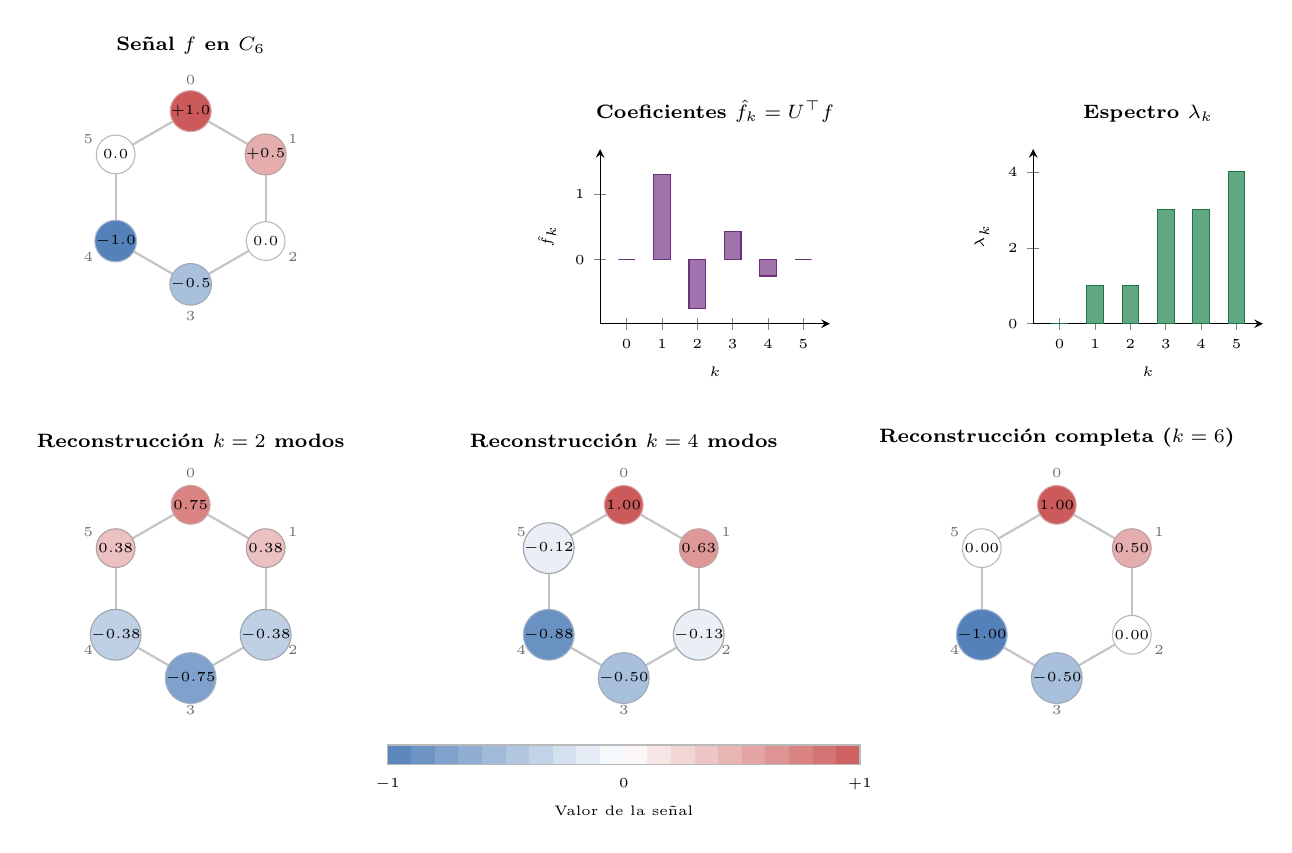
\begin{tikzpicture}

% === Row 1, Col 1: Signal on graph ===
\begin{scope}[shift={(0, 0)}]
  \node[anchor=south, font=\bfseries\scriptsize] at (0, 1.7) {Se\~nal $f$ en $C_6$};
  \draw[gdlgray!50, thick] (0.0000,1.1000) -- (0.9526,0.5500);
  \draw[gdlgray!50, thick] (0.9526,0.5500) -- (0.9526,-0.5500);
  \draw[gdlgray!50, thick] (0.9526,-0.5500) -- (0.0000,-1.1000);
  \draw[gdlgray!50, thick] (0.0000,-1.1000) -- (-0.9526,-0.5500);
  \draw[gdlgray!50, thick] (-0.9526,-0.5500) -- (-0.9526,0.5500);
  \draw[gdlgray!50, thick] (-0.9526,0.5500) -- (0.0000,1.1000);
  \node[circle, draw=gdlred!80!black!40, fill=gdlred!80!white, minimum size=14pt, inner sep=0pt, font=\tiny] (n0) at (0.0000,1.1000) {$+1.0$};
  \node[circle, draw=gdlred!40!black!40, fill=gdlred!40!white, minimum size=14pt, inner sep=0pt, font=\tiny] (n1) at (0.9526,0.5500) {$+0.5$};
  \node[circle, draw=gdlgray!60, fill=white, minimum size=14pt, inner sep=0pt, font=\tiny] (n2) at (0.9526,-0.5500) {$0.0$};
  \node[circle, draw=gdlblue!40!black!40, fill=gdlblue!40!white, minimum size=14pt, inner sep=0pt, font=\tiny] (n3) at (0.0000,-1.1000) {$-0.5$};
  \node[circle, draw=gdlblue!80!black!40, fill=gdlblue!80!white, minimum size=14pt, inner sep=0pt, font=\tiny] (n4) at (-0.9526,-0.5500) {$-1.0$};
  \node[circle, draw=gdlgray!60, fill=white, minimum size=14pt, inner sep=0pt, font=\tiny] (n5) at (-0.9526,0.5500) {$0.0$};
  \node[font=\tiny, text=gdlgray!80!black] at (0.0000,1.5000) {0};
  \node[font=\tiny, text=gdlgray!80!black] at (1.2990,0.7500) {1};
  \node[font=\tiny, text=gdlgray!80!black] at (1.2990,-0.7500) {2};
  \node[font=\tiny, text=gdlgray!80!black] at (0.0000,-1.5000) {3};
  \node[font=\tiny, text=gdlgray!80!black] at (-1.2990,-0.7500) {4};
  \node[font=\tiny, text=gdlgray!80!black] at (-1.2990,0.7500) {5};
\end{scope}

% === Row 1, Col 2: Fourier coefficients ===
\begin{scope}[shift={(5.2, -1.6)}]
  \begin{axis}[
    width=4.5cm, height=3.8cm,
    ybar,
    bar width=0.6em,
    title={\scriptsize\bfseries Coeficientes $\hat{f}_k = U^\top f$},
    xlabel={\tiny $k$},
    ylabel={\tiny $\hat{f}_k$},
    ymin=-0.98, ymax=1.69,
    xtick={0,1,2,3,4,5},
    xticklabel style={font=\tiny},
    yticklabel style={font=\tiny},
    xlabel style={font=\tiny},
    ylabel style={font=\tiny},
    title style={font=\scriptsize},
    tick label style={font=\tiny},
    axis lines=left,
    enlarge x limits=0.15,
  ]
    \addplot+[fill=barPurple, draw=barPurpleDark] coordinates {(0,-0.000000) (1,1.299038) (2,-0.750000) (3,0.433013) (4,-0.250000) (5,-0.000000)};
  \end{axis}
\end{scope}

% === Row 1, Col 3: Eigenvalue spectrum ===
\begin{scope}[shift={(10.7, -1.6)}]
  \begin{axis}[
    width=4.5cm, height=3.8cm,
    ybar,
    bar width=0.6em,
    title={\scriptsize\bfseries Espectro $\lambda_k$},
    xlabel={\tiny $k$},
    ylabel={\tiny $\lambda_k$},
    ymin=0.00, ymax=4.60,
    xtick={0,1,2,3,4,5},
    xticklabel style={font=\tiny},
    yticklabel style={font=\tiny},
    xlabel style={font=\tiny},
    ylabel style={font=\tiny},
    title style={font=\scriptsize},
    tick label style={font=\tiny},
    axis lines=left,
    enlarge x limits=0.15,
  ]
    \addplot+[fill=barGreen, draw=barGreenDark] coordinates {(0,-0.000000) (1,1.000000) (2,1.000000) (3,3.000000) (4,3.000000) (5,4.000000)};
  \end{axis}
\end{scope}

% === Row 2: Partial reconstructions ===
\begin{scope}[shift={(0.0, -5.0)}]
  \node[anchor=south, font=\bfseries\scriptsize] at (0, 1.7) {Reconstrucci\'on $k=2$ modos};
  \draw[gdlgray!50, thick] (0.0000,1.1000) -- (0.9526,0.5500);
  \draw[gdlgray!50, thick] (0.9526,0.5500) -- (0.9526,-0.5500);
  \draw[gdlgray!50, thick] (0.9526,-0.5500) -- (0.0000,-1.1000);
  \draw[gdlgray!50, thick] (0.0000,-1.1000) -- (-0.9526,-0.5500);
  \draw[gdlgray!50, thick] (-0.9526,-0.5500) -- (-0.9526,0.5500);
  \draw[gdlgray!50, thick] (-0.9526,0.5500) -- (0.0000,1.1000);
  \node[circle, draw=gdlred!60!black!40, fill=gdlred!60!white, minimum size=14pt, inner sep=0pt, font=\tiny] (n0) at (0.0000,1.1000) {$0.75$};
  \node[circle, draw=gdlred!30!black!40, fill=gdlred!30!white, minimum size=14pt, inner sep=0pt, font=\tiny] (n1) at (0.9526,0.5500) {$0.38$};
  \node[circle, draw=gdlblue!30!black!40, fill=gdlblue!30!white, minimum size=14pt, inner sep=0pt, font=\tiny] (n2) at (0.9526,-0.5500) {$-0.38$};
  \node[circle, draw=gdlblue!60!black!40, fill=gdlblue!60!white, minimum size=14pt, inner sep=0pt, font=\tiny] (n3) at (0.0000,-1.1000) {$-0.75$};
  \node[circle, draw=gdlblue!30!black!40, fill=gdlblue!30!white, minimum size=14pt, inner sep=0pt, font=\tiny] (n4) at (-0.9526,-0.5500) {$-0.38$};
  \node[circle, draw=gdlred!30!black!40, fill=gdlred!30!white, minimum size=14pt, inner sep=0pt, font=\tiny] (n5) at (-0.9526,0.5500) {$0.38$};
  \node[font=\tiny, text=gdlgray!80!black] at (0.0000,1.5000) {0};
  \node[font=\tiny, text=gdlgray!80!black] at (1.2990,0.7500) {1};
  \node[font=\tiny, text=gdlgray!80!black] at (1.2990,-0.7500) {2};
  \node[font=\tiny, text=gdlgray!80!black] at (0.0000,-1.5000) {3};
  \node[font=\tiny, text=gdlgray!80!black] at (-1.2990,-0.7500) {4};
  \node[font=\tiny, text=gdlgray!80!black] at (-1.2990,0.7500) {5};
\end{scope}
\begin{scope}[shift={(5.5, -5.0)}]
  \node[anchor=south, font=\bfseries\scriptsize] at (0, 1.7) {Reconstrucci\'on $k=4$ modos};
  \draw[gdlgray!50, thick] (0.0000,1.1000) -- (0.9526,0.5500);
  \draw[gdlgray!50, thick] (0.9526,0.5500) -- (0.9526,-0.5500);
  \draw[gdlgray!50, thick] (0.9526,-0.5500) -- (0.0000,-1.1000);
  \draw[gdlgray!50, thick] (0.0000,-1.1000) -- (-0.9526,-0.5500);
  \draw[gdlgray!50, thick] (-0.9526,-0.5500) -- (-0.9526,0.5500);
  \draw[gdlgray!50, thick] (-0.9526,0.5500) -- (0.0000,1.1000);
  \node[circle, draw=gdlred!80!black!40, fill=gdlred!80!white, minimum size=14pt, inner sep=0pt, font=\tiny] (n0) at (0.0000,1.1000) {$1.00$};
  \node[circle, draw=gdlred!50!black!40, fill=gdlred!50!white, minimum size=14pt, inner sep=0pt, font=\tiny] (n1) at (0.9526,0.5500) {$0.63$};
  \node[circle, draw=gdlblue!30!black!40, fill=gdlblue!10!white, minimum size=14pt, inner sep=0pt, font=\tiny] (n2) at (0.9526,-0.5500) {$-0.13$};
  \node[circle, draw=gdlblue!40!black!40, fill=gdlblue!40!white, minimum size=14pt, inner sep=0pt, font=\tiny] (n3) at (0.0000,-1.1000) {$-0.50$};
  \node[circle, draw=gdlblue!70!black!40, fill=gdlblue!70!white, minimum size=14pt, inner sep=0pt, font=\tiny] (n4) at (-0.9526,-0.5500) {$-0.88$};
  \node[circle, draw=gdlblue!30!black!40, fill=gdlblue!10!white, minimum size=14pt, inner sep=0pt, font=\tiny] (n5) at (-0.9526,0.5500) {$-0.12$};
  \node[font=\tiny, text=gdlgray!80!black] at (0.0000,1.5000) {0};
  \node[font=\tiny, text=gdlgray!80!black] at (1.2990,0.7500) {1};
  \node[font=\tiny, text=gdlgray!80!black] at (1.2990,-0.7500) {2};
  \node[font=\tiny, text=gdlgray!80!black] at (0.0000,-1.5000) {3};
  \node[font=\tiny, text=gdlgray!80!black] at (-1.2990,-0.7500) {4};
  \node[font=\tiny, text=gdlgray!80!black] at (-1.2990,0.7500) {5};
\end{scope}
\begin{scope}[shift={(11.0, -5.0)}]
  \node[anchor=south, font=\bfseries\scriptsize] at (0, 1.7) {Reconstrucci\'on completa ($k=6$)};
  \draw[gdlgray!50, thick] (0.0000,1.1000) -- (0.9526,0.5500);
  \draw[gdlgray!50, thick] (0.9526,0.5500) -- (0.9526,-0.5500);
  \draw[gdlgray!50, thick] (0.9526,-0.5500) -- (0.0000,-1.1000);
  \draw[gdlgray!50, thick] (0.0000,-1.1000) -- (-0.9526,-0.5500);
  \draw[gdlgray!50, thick] (-0.9526,-0.5500) -- (-0.9526,0.5500);
  \draw[gdlgray!50, thick] (-0.9526,0.5500) -- (0.0000,1.1000);
  \node[circle, draw=gdlred!80!black!40, fill=gdlred!80!white, minimum size=14pt, inner sep=0pt, font=\tiny] (n0) at (0.0000,1.1000) {$1.00$};
  \node[circle, draw=gdlred!40!black!40, fill=gdlred!40!white, minimum size=14pt, inner sep=0pt, font=\tiny] (n1) at (0.9526,0.5500) {$0.50$};
  \node[circle, draw=gdlgray!60, fill=white, minimum size=14pt, inner sep=0pt, font=\tiny] (n2) at (0.9526,-0.5500) {$0.00$};
  \node[circle, draw=gdlblue!40!black!40, fill=gdlblue!40!white, minimum size=14pt, inner sep=0pt, font=\tiny] (n3) at (0.0000,-1.1000) {$-0.50$};
  \node[circle, draw=gdlblue!80!black!40, fill=gdlblue!80!white, minimum size=14pt, inner sep=0pt, font=\tiny] (n4) at (-0.9526,-0.5500) {$-1.00$};
  \node[circle, draw=gdlgray!60, fill=white, minimum size=14pt, inner sep=0pt, font=\tiny] (n5) at (-0.9526,0.5500) {$0.00$};
  \node[font=\tiny, text=gdlgray!80!black] at (0.0000,1.5000) {0};
  \node[font=\tiny, text=gdlgray!80!black] at (1.2990,0.7500) {1};
  \node[font=\tiny, text=gdlgray!80!black] at (1.2990,-0.7500) {2};
  \node[font=\tiny, text=gdlgray!80!black] at (0.0000,-1.5000) {3};
  \node[font=\tiny, text=gdlgray!80!black] at (-1.2990,-0.7500) {4};
  \node[font=\tiny, text=gdlgray!80!black] at (-1.2990,0.7500) {5};
\end{scope}

% === Color legend ===
\begin{scope}[shift={(0, -7.2)}]
  \fill[gdlblue!76!white] (2.500, 0) rectangle (2.800, 0.25);
  \fill[gdlblue!68!white] (2.800, 0) rectangle (3.100, 0.25);
  \fill[gdlblue!60!white] (3.100, 0) rectangle (3.400, 0.25);
  \fill[gdlblue!52!white] (3.400, 0) rectangle (3.700, 0.25);
  \fill[gdlblue!44!white] (3.700, 0) rectangle (4.000, 0.25);
  \fill[gdlblue!36!white] (4.000, 0) rectangle (4.300, 0.25);
  \fill[gdlblue!28!white] (4.300, 0) rectangle (4.600, 0.25);
  \fill[gdlblue!20!white] (4.600, 0) rectangle (4.900, 0.25);
  \fill[gdlblue!12!white] (4.900, 0) rectangle (5.200, 0.25);
  \fill[gdlblue!4!white] (5.200, 0) rectangle (5.500, 0.25);
  \fill[gdlred!4!white] (5.500, 0) rectangle (5.800, 0.25);
  \fill[gdlred!12!white] (5.800, 0) rectangle (6.100, 0.25);
  \fill[gdlred!20!white] (6.100, 0) rectangle (6.400, 0.25);
  \fill[gdlred!28!white] (6.400, 0) rectangle (6.700, 0.25);
  \fill[gdlred!36!white] (6.700, 0) rectangle (7.000, 0.25);
  \fill[gdlred!44!white] (7.000, 0) rectangle (7.300, 0.25);
  \fill[gdlred!52!white] (7.300, 0) rectangle (7.600, 0.25);
  \fill[gdlred!60!white] (7.600, 0) rectangle (7.900, 0.25);
  \fill[gdlred!68!white] (7.900, 0) rectangle (8.200, 0.25);
  \fill[gdlred!76!white] (8.200, 0) rectangle (8.500, 0.25);
  \draw[gdlgray!60] (2.500, 0) rectangle (8.500, 0.25);
  \node[font=\tiny, anchor=north] at (2.500, -0.05) {$-1$};
  \node[font=\tiny, anchor=north] at (5.500, -0.05) {$0$};
  \node[font=\tiny, anchor=north] at (8.500, -0.05) {$+1$};
  \node[font=\tiny, anchor=north] at (5.500, -0.4) {Valor de la se\~nal};
\end{scope}

\end{tikzpicture}
\end{document}